%\documentclass[a4paper,12pt,twoside]{report}
\documentclass[a4paper,12pt]{report}

\usepackage{url}
\usepackage{amsmath}
\usepackage{lipsum}
\usepackage{listings}
\usepackage{color}
\usepackage{graphicx}

\definecolor{mygreen}{rgb}{0,0.6,0}
\definecolor{mygray}{rgb}{0.6,0.6,0.6}
\definecolor{mymauve}{rgb}{0.58,0,0.82}

\lstset{
  captionpos=b,
  numbers=left,
  frame=tb,
  showstringspaces=false,
  numbersep=15pt,
  xleftmargin=30pt,
  aboveskip=15pt,
  belowskip=15pt,
  keywordstyle=\color{blue},
  stringstyle=\color{mymauve},
  numberstyle=\color{mygray},
  rulecolor=\color{mygray}
}

\title{Resolution of two dimensional collisions}
\author{Philip Burridge\\
        Dan Camarda\\
        Alexander Cederblad\\
        Rasmus Haapaoja\\
        Fredrik Johnson}
\date{\today}


%-- Document
\begin{document}


%-- Title
\maketitle


%-- Abstract
\begin{abstract}
Cum M.~Cicero consul Nonis Decembribus senatum in aede Iovis Statoris consuleret, quid de iis coniurationis Catilinae sociis fieri placeret, qui in custodiam traditi essent, factum est, ut duae potissimum sententiae proponerentur, una D.~Silani consulis designati, qui morte multandos illos censebat\cite{gdm}.
\end{abstract}


%-- Table of Contents
\tableofcontents
%\listoffigures
%\listoftables
%\lstlistoflistings


%-- Introduction
\chapter{Introduction}
\setcounter{page}{1}

\lipsum[0-1]

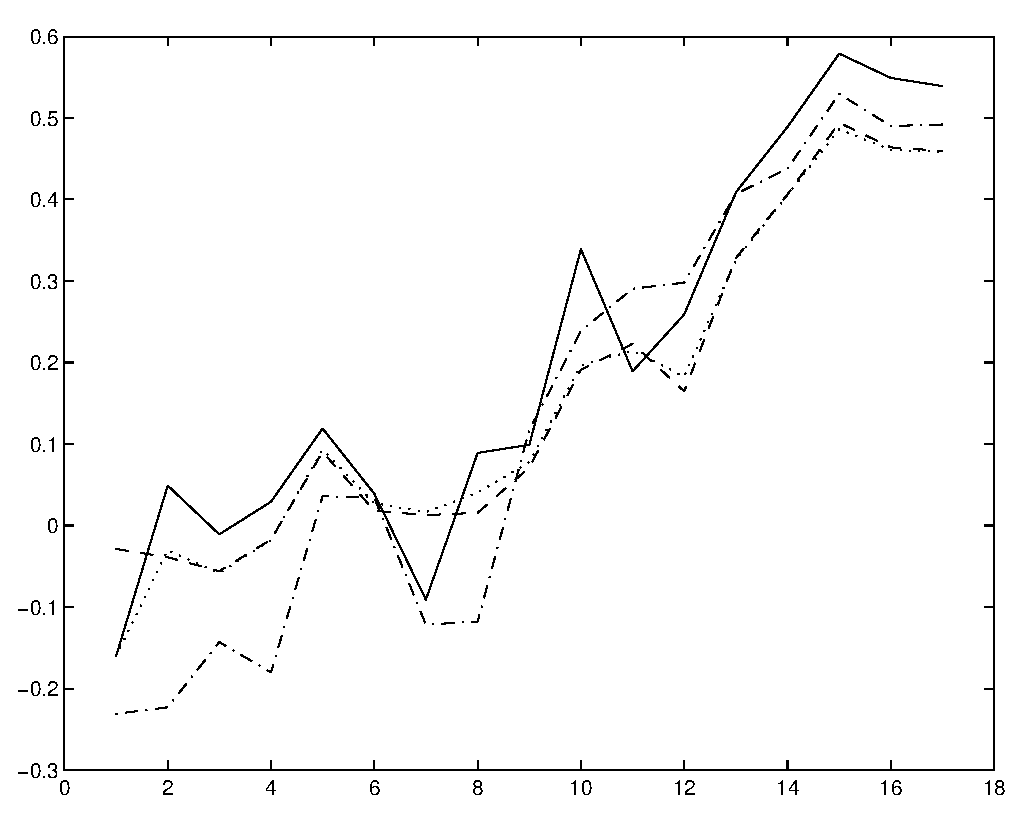
\includegraphics[scale=0.5]{figures/result.eps}

\lipsum[0-1]


%-- Method
\chapter{Method}

% Collision detection
\section{Collision detection}

\lipsum[0-2]

% Resolvning an impulse
\section{Resolving an impulse}
\begin{equation}
j = \dfrac{ -(1+e) \mathbf v_{AB} \cdot \mathbf n }{
    \mathbf n \cdot \mathbf n ( \dfrac{1}{M_{A}} + \dfrac{1}{M_{A}} )
    + \dfrac{ (\mathbf r_{AP\perp} \cdot \mathbf n)^2}{I_{A} }
    + \dfrac{ (\mathbf r_{BP\perp} \cdot \mathbf n)^2}{I_{B} } }
\label{e1}
\end{equation}

\lipsum[0-1]

\begin{equation}
\mathbf v'_{A}=\mathbf v'_{A}+\frac{j}{M_{A}}\mathbf n
\label{e2}
\end{equation}
\begin{equation}
\omega'_{A}=\omega'_{A}+\frac{\mathbf r_{AP\perp}\cdot j\mathbf n}{I_{A}}
\label{e3}
\end{equation}

\lipsum[0-1]

% Resolvning an impulse
\section{Numerical integration}

\lipsum[0-1]

\begin{equation}
y_{n+1}=y_{n}+hf(t_n, y_n)
\label{e4}
\end{equation}

% OpenGL Implementation
\section{OpenGL implementation}

\lipsum[0-1]

\begin{lstlisting}[caption={This is a Hello World application written in C++.}, language={C++}]
#include <iostream>

int main(int argc, char **argv)
{
    std::cout << "Hello world!" << std::endl;
    return 0;
}
\end{lstlisting}

\subsection{Running the simulation}
Navigate to the folder with your current operating system and click the executable file named $simulation$ to run the simulation. The software is not tested on any Linux distribution.

\subsubsection{Requirements}
\begin{itemize}
    \item Graphics card from this century
\end{itemize}


%-- Discussion
\chapter{Discussion}

\lipsum[0-1]


%-- Bibliography
\bibliographystyle{vancouver}
\bibliography{report}


%-- End of Document
\end{document}

